\documentclass{beamer}

\usepackage[game]{sfocs-slides}
\author{Team $13$: Zining Wang, Yifan Jia, Qiao Liu.}
\title{Terminator}
\date{Summer 2021}

\begin{document}

\maketitle

\section{Background Story}

\begin{frame}{Background Story}
	
	\begin{columns}
			\column{\halfwidth}
			\fadedpic[width=\textwidth]{open}{}
			\column{\halfwidth}
			\fadedpic[width=\textwidth]{open2}{}
		\end{columns}
		\pause
   \centering \textbf{{Horrible Pandemic Sweeping In!\\}}
\vspace{0.5cm}
	Four districts in a coastal metropolis LosSantos stricken by a horrible pandemic VOPID-141 is in utter chaos. Citizen’s lives and the urban resources are at stake in Gotham, Bombay, GassVille, Burnley! Out of humanistic concern, the only way to get through this is...



\end{frame}

\begin{frame}{Background Story}

	\begin{tikzpicture}[overlay, remember picture]

		\node[anchor=south west,outer sep=0pt,inner sep=0pt] (c1) at (current page.south west)  {
\includegraphics[height=\heightiii]{arn28-kj5eh.png}};
		\node[anchor=south west,outer sep=0pt,inner sep=0pt] at (c1.north west) (c2) {
\includegraphics[height=\heightiii]{ai97b-ej97b.png}};
		\node[anchor=south west,outer sep=0pt,inner sep=0pt] at (c2.north west) {\includegraphics[height=\heightiii]{截屏2021-07-22 11.58.10-2.png}};

	\end{tikzpicture}
	\begin{columns}
		\column{.22\textwidth}

		\column{.7275\textwidth}
	
		\begin{itemize}\bigsep
			\item Appointed as the Mayor
			\item You will be the terminator of the pandemic!
		\end{itemize}
	\end{columns}

\end{frame}


\section{Game Play}
\begin{frame}{Game Play}
	\begin{tikzpicture}[overlay, remember picture]

		\node[anchor=south west,outer sep=0pt,inner sep=0pt] (c1) at (current page.south west)  {\includegraphics[height=\heightiii]{sc3}};
		\node[anchor=south west,outer sep=0pt,inner sep=0pt] at (c1.north west) (c2) {\includegraphics[height=\heightiii]{sc2}};
		\node[anchor=south west,outer sep=0pt,inner sep=0pt] at (c2.north west) {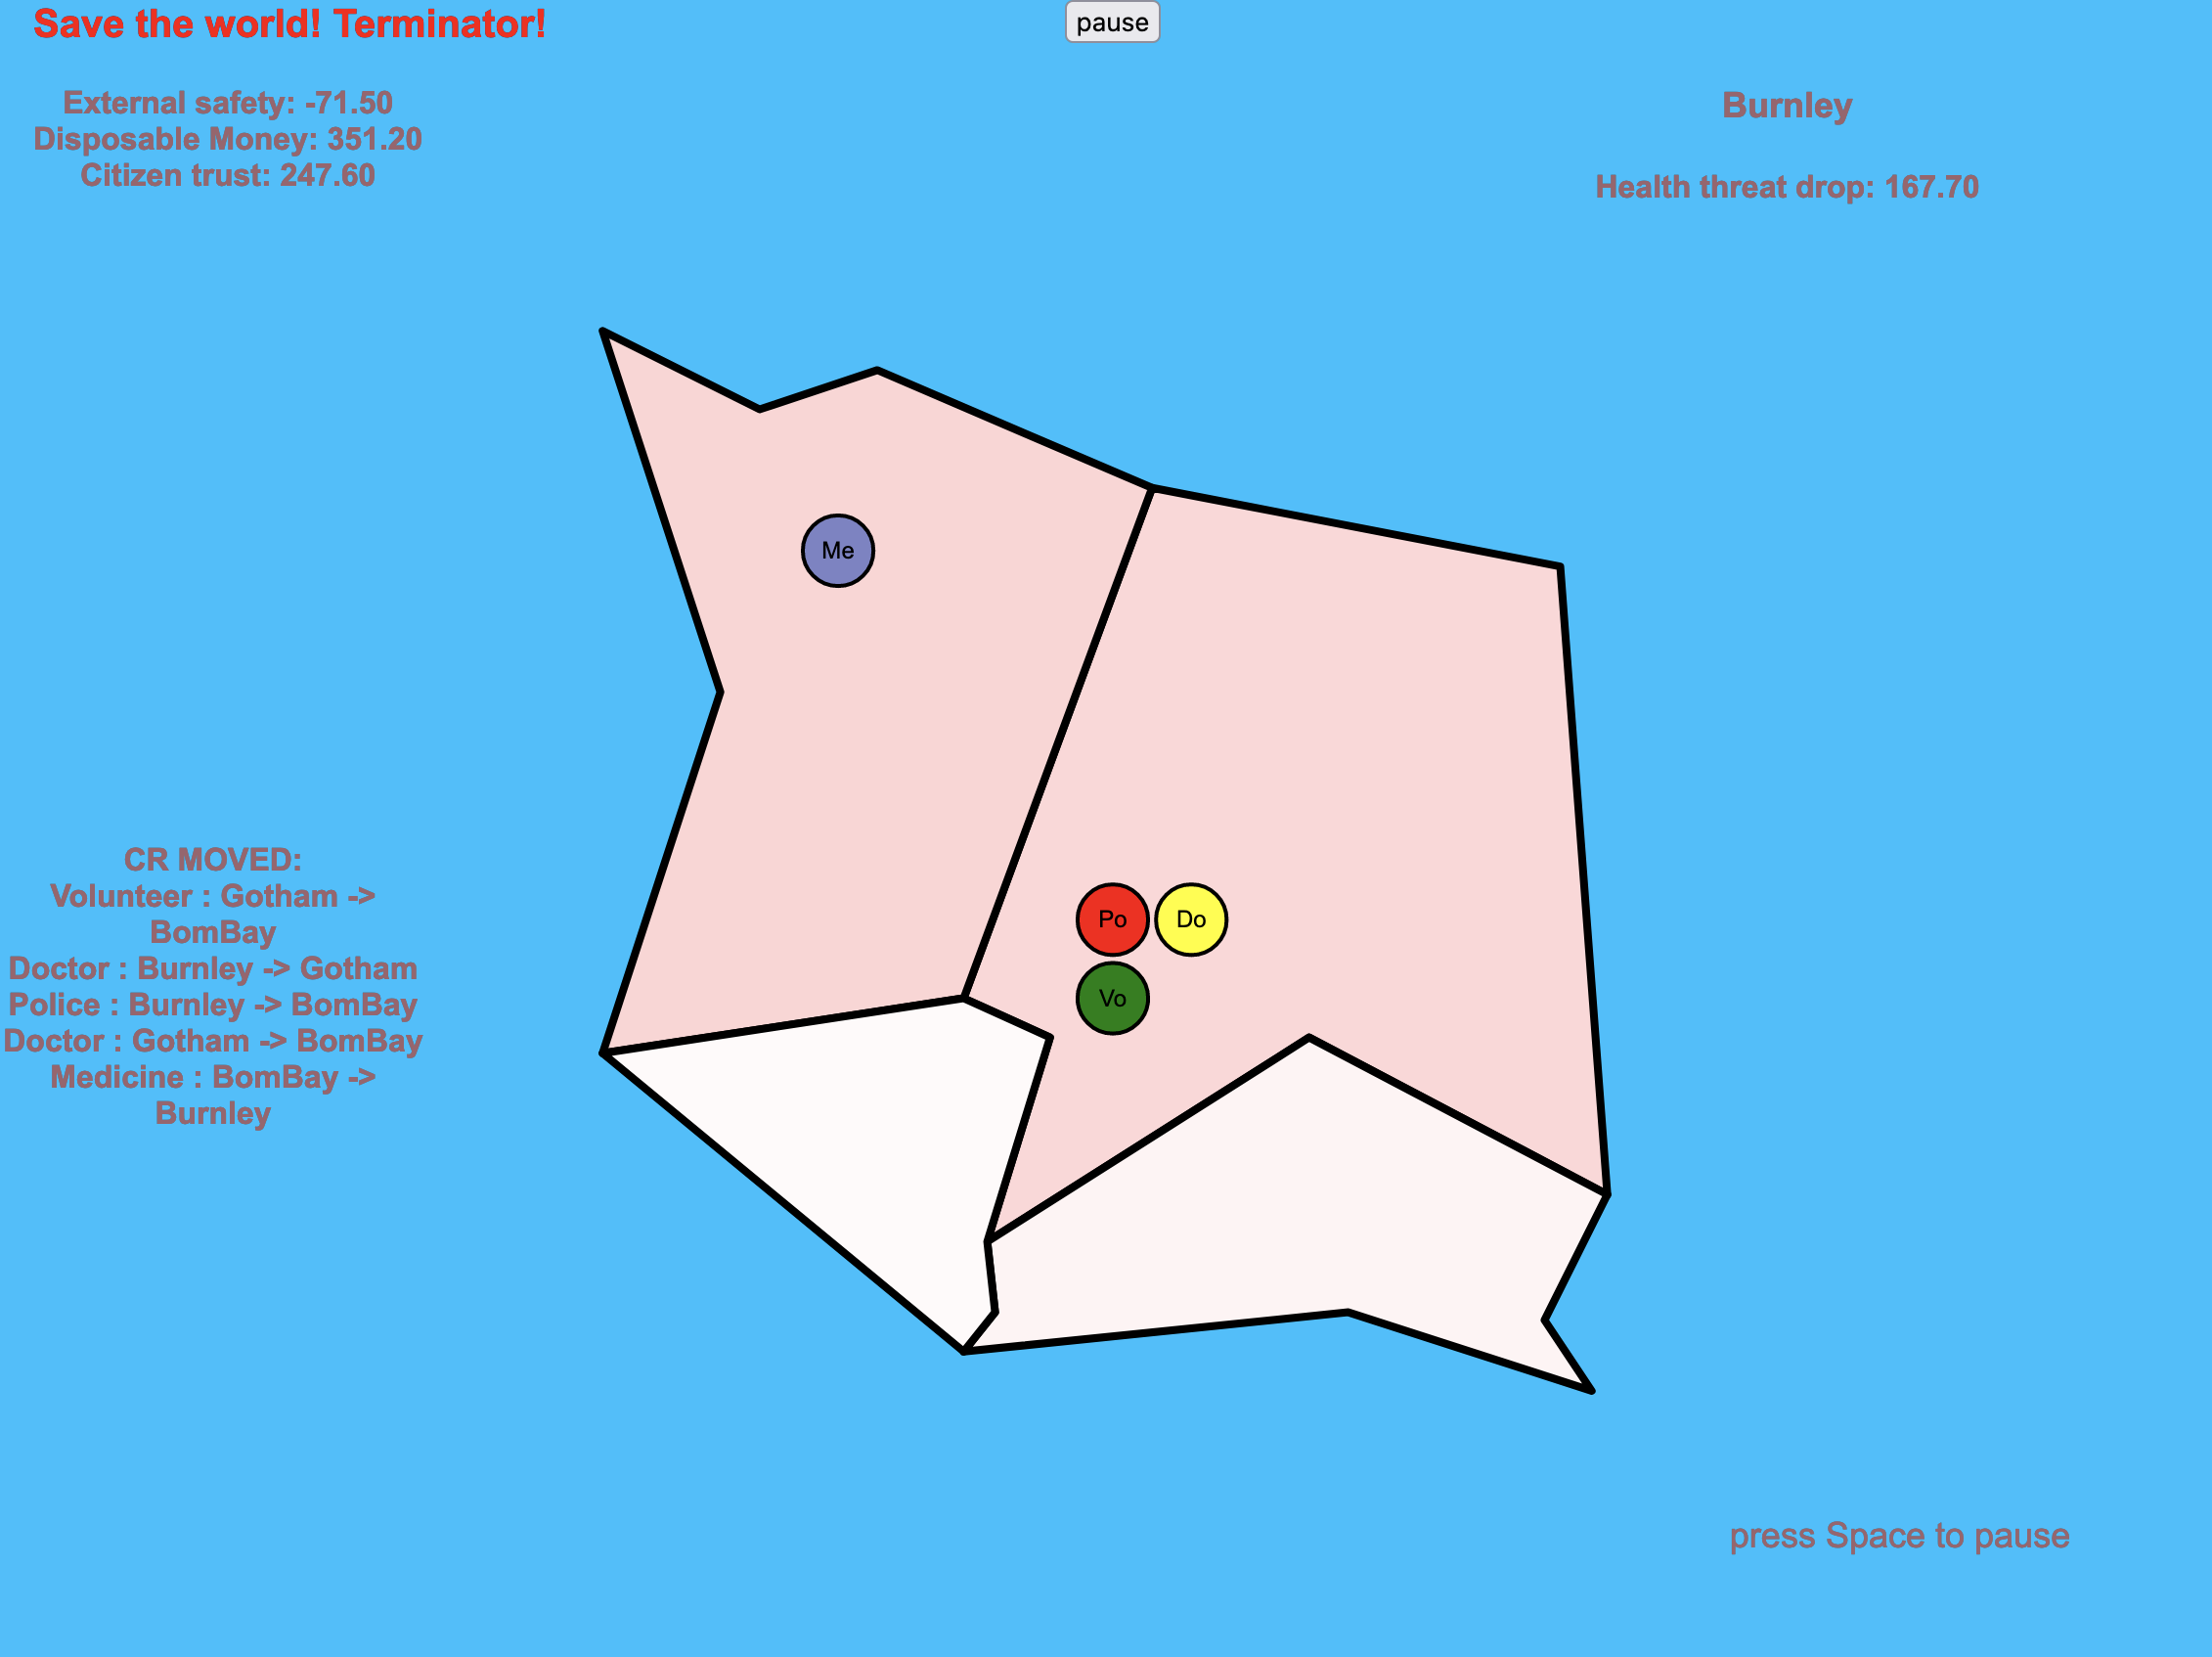
\includegraphics[height=\heightiii]{sc1}};

	\end{tikzpicture}
	\begin{columns}
		\column{.22\textwidth}

		\column{.7275\textwidth}
		\begin{itemize}\bigsep
			\item The shade of the color changes
			\item It indicate the urgency of the district
			\item More control point loss leads to higher urgency
			\item The district's status update every few seconds
		\end{itemize}
	\end{columns}
\end{frame}


\section{Game Controlling}

\begin{frame}{Game Controlling}
	\begin{tikzpicture}[overlay, remember picture]


	
		\node[anchor=west,outer sep=0pt,inner sep=0pt] at (c2.west) {\includegraphics[height=\heightiii]{WechatIMG10657.png}};

	\end{tikzpicture}
\begin{columns}
		\column{.22\textwidth}

		\column{.7275\textwidth}
		Simple Operations:
	\begin{itemize}\bigsep
		\item Click on the colorful dots in a district
		\item Then click on another target district
		\item A transference of Critical Resources is made
		\item Check how the control points have changed
	\end{itemize}
	\end{columns}
\end{frame}

\section{Reference}

\begin{frame}{Reference}

	Graphics:
	\begin{itemize}\bigsep
		\item The Corona Virus: by iXimus from Pixabay
		\item The injection needle: by Memed Nurrohmad from Pixabay
		\item The politician: by OpenClipart-Vectors from Pixabay
		\item The doctor: OpenClipart-Vectors from Pixabay
	\end{itemize}

\end{frame}




\begin{framek}

\begin{itemize}\itemsep .5cm
		\item Highly Customized User Control
		\item Simple yet Ingenious Operation
		\item Minimalist User Interface
		\item The Humanism Concept
		\item Accessible on mobile phones
		\item Game Mod Diversity
	\end{itemize}

\end{framek}

\end{document}
